\documentclass[a5paper, 10pt]{article}

% Текст
\usepackage[utf8]{inputenc} % UTF-8 кодировка
\usepackage[russian]{babel} % Русский язык
\usepackage{indentfirst} % красная строка в первом параграфе в главе
% Отображение страниц
\usepackage{geometry} % размеры листа и отступов
\usepackage{listings}
\usepackage{color}

\geometry{
	left=12mm,
	top=25mm,
	right=15mm,
	bottom=17mm,
	marginparsep=0mm,
	marginparwidth=0mm,
	headheight=10mm,
	headsep=7mm,
	nofoot}
\usepackage{afterpage,fancyhdr} % настройка колонтитулов
\pagestyle{fancy}
\fancypagestyle{style}{ % создание нового стиля style
	\fancyhf{} % очистка колонтитулов
	\fancyhead[LO, RE]{Лабораторная работа № 4 } % название документа наверху
	\fancyhead[RO, LE]{Динамические системы} % название section наверху
	\fancyfoot[RO, LE]{\thepage} % номер страницы справа внизу на нечетных и слева внизу на четных
	\renewcommand{\headrulewidth}{0.25pt} % толщина линии сверху
	\renewcommand{\footrulewidth}{0pt} % толцина линии снизу
}
\fancypagestyle{plain}{ % создание нового стиля plain -- полностью пустого
	\fancyhf{}
	\renewcommand{\headrulewidth}{0pt}
}
\fancypagestyle{title}{ % создание нового стиля title -- для титульной страницы
	\fancyhf{}
	\fancyhead[C]{{\footnotesize
			Министерство образования и науки Российской Федерации\\
			Федеральное государственное автономное образовательное учреждение высшего образования
	}}
	\fancyfoot[C]{{\large 
			Санкт-Петербург, 2023-2024
	}}
	\renewcommand{\headrulewidth}{0pt}
}

% Математика
\usepackage{amsmath, amsfonts, amssymb, amsthm} % Набор пакетов для математических текстов
%\usepackage{dmvnbase} % мехматовский пакет latex-сокращений
\usepackage{cancel} % зачеркивание для сокращений
% Рисунки и фигуры
\usepackage[pdftex]{graphicx} % вставка рисунков
\usepackage{wrapfig, subcaption} % вставка фигур, обтекая текст
\usepackage{caption} % для настройки подписей
\captionsetup{figurewithin=none,labelsep=period, font={small,it}} % настройка подписей к рисункам
% Рисование
\usepackage{tikz} % рисование
\usepackage{circuitikz}
\usepackage{pgfplots} % графики
% Таблицы
\usepackage{multirow} % объединение строк
\usepackage{multicol} % объединение столбцов
% Остальное
\usepackage[unicode, pdftex]{hyperref} % гиперссылки
\usepackage{enumitem} % нормальное оформление списков
\setlist{itemsep=0.15cm,topsep=0.15cm,parsep=1pt} % настройки списков
% Теоремы, леммы, определения...
\theoremstyle{definition}
\newtheorem{Def}{Определение}
\newtheorem*{Axiom}{Аксиома}
\theoremstyle{plain}
\newtheorem{Th}{Теорема}
\newtheorem{Lem}{Лемма}
\newtheorem{Cor}{Следствие}
\newtheorem{Ex}{Пример}
\theoremstyle{remark}
\newtheorem*{Note}{Замечание}
\newtheorem*{Solution}{Решение}
\newtheorem*{Proof}{Доказательство}
% Свои команды
\newcommand{\comb}[1]{\left[\hspace{-4pt}\begin{array}{l}#1\end{array}\right.\hspace{-5pt} } % совокупность уравнений
% Титульный лист
\usepackage{csvsimple-l3}
\newcommand*{\titlePage}{
	\thispagestyle{title}
	\begingroup
	\begin{center}
		%		{\footnotesize
			%			Министерство образования и науки Российской Федерации\\
			%			Федеральное государственное автономное образовательное учреждение высшего образования
			%		}
		%		
		\vspace*{6ex}
		
		{\small
			САНКТ-ПЕТЕРБУРГСКИЙ НАЦИОНАЛЬНЫЙ ИССЛЕДОВАТЕЛЬСКИЙ УНИВЕРСИТЕТ ИТМО	
		}
		
		\vspace*{2ex}
		
		{\normalsize
			Факультет систем управления и робототехники
		}
		
		\vspace*{15ex}
		
		{\Large \bfseries 
			Лабораторная работа № 4
		}
\vspace*{2ex}
	{\Large \bfseries 
			
"Динамические системы"
		}
\vspace*{2ex}
		
		{\normalsize
			по дисциплине Практическая линейная алгебра
		}

	\end{center}
	\vspace*{20ex}
	\begin{flushright}
		{\large 
			\underline{Выполнила}: студентка гр. \textbf{R3238}\\
			\begin{flushright}
				\textbf{Нечаева А. А.}\\
			\end{flushright}
		}
		
		\vspace*{5ex}
		
		{\large 
			\underline{Преподаватель}: \textit{Перегудин Алексей Алексеевич}
		}
	\end{flushright}	
	\newpage
	\setcounter{page}{1}
	\endgroup}

\begin{document}
	\titlePage
	\pagestyle{style}
\newpage
\textit{В этой лабораторной мы будем работать с непрерывными $ \left( t \in \mathbb{R} \right) $ и дискретными $ \left( k \in \mathbb{Z} \right)$  линейными динамическими системами второго порядка вида}

\begin{equation}
\begin{cases}
\dot{x}_1(t) = a_1x_1(t)+a_2x_2(t),\\
\dot{x}_2(t) = a_3x_1(t)+a_4x_2(t)
\end{cases}
\end{equation}

\begin{equation}
\begin{cases}
x_1(k+1) = a_1x_1(k)+a_2x_2(k),\\
x_2(k+1) = a_3x_1(k)+a_4x_2(k)
\end{cases}
\end{equation}
в более компактной форме:
\begin{equation}
\dot{x}(t) = Ax(t),
\end{equation}

\begin{equation}
x(k+1) = Ax(k),
\end{equation}
где $x(\cdot) \in  \mathbb{R}^2, \,  \mathbb{R}^{2 \times 2} $.

\newpage
\section{задание. Придумать непрерывное.}
Зададимся двумя неколлинеарными векторами $v_1, \, v_2 \in \mathbb{R}^2$, не лежащими на координатных осях:
\begin{equation}
v_1 =
\begin{pmatrix}
1\\
4\\
\end{pmatrix}
\, \, \, \, \, \, \, \, \, \,
v_2 =
\begin{pmatrix}
2\\
3\\
\end{pmatrix}
\end{equation}
Придумаем непрерывные динамические системы:

% part 1
\subsection{}
\textit{Система ассимптотически устойчива, при этом если $x(0) = v_1$, то $x(t) \in Span\{v_1\}$, а если $x(0) = v_2,$ то  $x(t) \in Span\{v_2\}$ при всех $t \geq 0$.}\\
\\
Обратимся к уравнению $\dot{x}(t)=Ax(t), \, \, \, x(0) = x_0$ и к его решению:\\ $x(t) = e^{At}x_0$.\\
\\
1. Система асимптотически устойчива, значит выполнено $\lim \limits_{t \to \infty} x(t) = 0$.
\\
2. Выберем матрицу с двумя совпадающими \textbf{отрицательными} собственными числами, например:
\begin{equation}
A=
\begin{pmatrix}
-1 & 0\\
0 & -1
\end{pmatrix}
\end{equation}
Собственные числа $\lambda_1 = \lambda_2 = -1$,\\ собственные векторы $w_1 = \begin{pmatrix} a \\ 0 \end{pmatrix}$,  $w_2 = \begin{pmatrix} 0 \\ b \end{pmatrix}$, $a, b \in \mathbb{R}$.




% part 2
\subsection{}
\textit{Система неустойчива, при этом у матрицы $A$ не существует двух неколлинеарных собственных векторов.}
\begin{equation}
A=
\begin{pmatrix}
4 & 1\\
0 & 4
\end{pmatrix}
\end{equation}

Собственные числа: $\lambda_1 = 4, \, \lambda_2 = 4$, собственные векторы соответственно $w_1 = \begin{pmatrix} a \\ 0 \end{pmatrix}$,  $w_2 = \begin{pmatrix} b \\ 0 \end{pmatrix}$, $a, b \in \mathbb{R}$.


% part 3
\subsection{}
\textit{Система неустойчива, при этом если $x(0) = v_1$, то $\lim\limits_{t \to \infty} x(t) = 0$.}
\begin{equation}
A=
\begin{pmatrix}
0 & -1\\
-16 & 0
\end{pmatrix}
\end{equation}
Собственные числа: $\lambda_1 = 4, \, \lambda_2 = -4$, собственные векторы соответственно $w_1 = \begin{pmatrix} -1 \\ 4 \end{pmatrix}$,  $w_2 = \begin{pmatrix} 1 \\ 4 \end{pmatrix}$.

% part 4
\subsection{}
\textit{Система асимптотически устойчива, при этом матрица $A \in \mathbb{R}^2$ имеет комплексные собственные вектора вида $v_1 \pm v_2 i \in \mathbb{C}^2$.}\\
\\
Сначала запишем собственные векторы искомой матрицы:
\begin{equation}
w_1 =
\begin{pmatrix}
1 + 2i \\
4 + 3i
\end{pmatrix}
\,\,\,\,\,\,\,\,\,\,
w_2 =
\begin{pmatrix}
1 - 2i \\
4 - 3i
\end{pmatrix}
\end{equation}

Будем искать матрицу записав ее спектральное разложение $ A = V \cdot D \cdot V^{-1}$, где $V$ -- матрица, составленная из собственных векторов матрицы $A$, $D$ -- матрица, на главной диагонали которой расположены собственные числа.

\begin{equation}
A =
\begin{pmatrix}
1 + 2i &  1 - 2i \\
4 + 3i & 4 - 3i
\end{pmatrix}
\begin{pmatrix}
-1 + i &  0 \\
0 & -1 -i
\end{pmatrix}
\begin{pmatrix}
1 + 2i &  1 - 2i \\
4 + 3i & 4 - 3i
\end{pmatrix}^{-1}
=
\begin{pmatrix}
1 & -1  \\
5 & -3
\end{pmatrix}
\end{equation}
Искомая матрица:
\begin{equation}
A =
\begin{pmatrix}
1 & -1  \\
5 & -3
\end{pmatrix}
\end{equation}

% part 5
\subsection{}
\textit{Система неустойчива, при этом матрица $A$ имеет такие же слбственные вектора, как в предыдущем пункте.}\\
\\
Аналогично будем искать матрицу записав ее спектральное разложение $ A = V \cdot D \cdot V^{-1}$, где $V$ -- матрица, составленная из собственных векторов матрицы $A$, $D$ -- матрица, на главной диагонали которой расположены собственные числа.

\begin{equation}
A =
\begin{pmatrix}
1 + 2i &  1 - 2i \\
4 + 3i & 4 - 3i
\end{pmatrix}
\begin{pmatrix}
1+ i &  0 \\
0 & 1 -i
\end{pmatrix}
\begin{pmatrix}
1 + 2i &  1 - 2i \\
4 + 3i & 4 - 3i
\end{pmatrix}^{-1}
=
\begin{pmatrix}
3 & -1  \\
5 & -1
\end{pmatrix}
\end{equation}
Искомая матрица:
\begin{equation}
A =
\begin{pmatrix}
3 & -1  \\
5 & -1
\end{pmatrix}
\end{equation}


% part 6
\subsection{}
\textit{Система не является асимптотически устойчивой, но не является и неустойчивой, при этом матрица $A$ имеет собственные векторы такие же, как в пункте 4.}\\

Вновь будем искать матрицу записав ее спектральное разложение $ A = V \cdot D \cdot V^{-1}$, где $V$ -- матрица, составленная из собственных векторов матрицы $A$, $D$ -- матрица, на главной диагонали которой расположены собственные числа.

\begin{equation}
A =
\begin{pmatrix}
1 + 2i &  1 - 2i \\
4 + 3i & 4 - 3i
\end{pmatrix}
\begin{pmatrix}
i &  0 \\
0 & -i
\end{pmatrix}
\begin{pmatrix}
1 + 2i &  1 - 2i \\
4 + 3i & 4 - 3i
\end{pmatrix}^{-1}
=
\begin{pmatrix}
2 & -1  \\
5 & -2
\end{pmatrix}
\end{equation}
Искомая матрица:
\begin{equation}
A =
\begin{pmatrix}
2 & -1  \\
5 & -2
\end{pmatrix}
\end{equation}


%task 2
\newpage
\section{задание. Замоделировать непрерывное.}

% part 1
\subsection{}
\textit{Система ассимптотически устойчива, при этом если $x(0) = v_1$, то $x(t) \in Span\{v_1\}$, а если $x(0) = v_2,$ то  $x(t) \in Span\{v_2\}$ при всех $t \geq 0$.}
\begin{equation}
A=
\begin{pmatrix}
-1 & 0\\
0 & -1
\end{pmatrix}
\end{equation}

\begin{figure}[h!]
\center{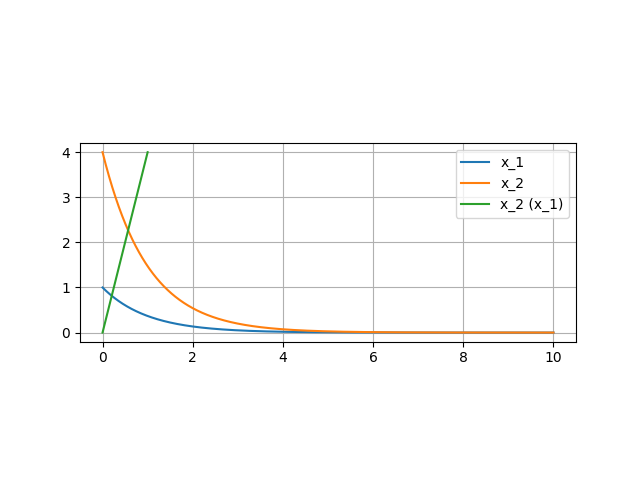
\includegraphics[width=1\linewidth]{pic/1_x0_1_4_single.png}}
\caption{Моделирование при $x_0 = \begin{pmatrix} 1 \\ 4 \end{pmatrix}$.}
\end{figure}

\begin{figure}[h!]
\center{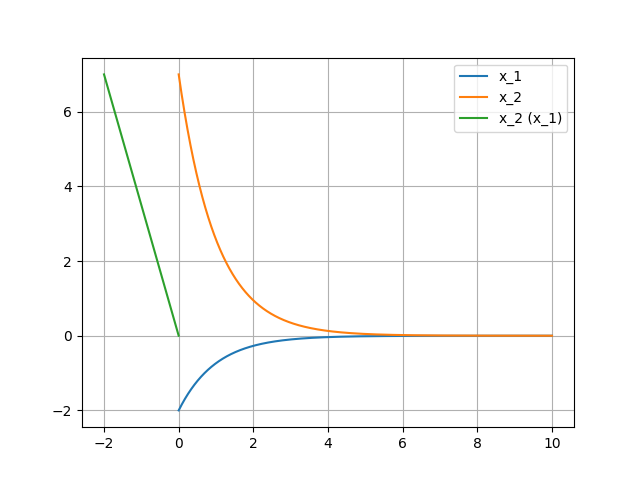
\includegraphics[width=0.7\linewidth]{pic/1_x0_2_s.png}}
\caption{Моделирование при $x_0 = \begin{pmatrix} -2 \\ 7 \end{pmatrix}$.}
\end{figure}
\begin{figure}[h!]
\center{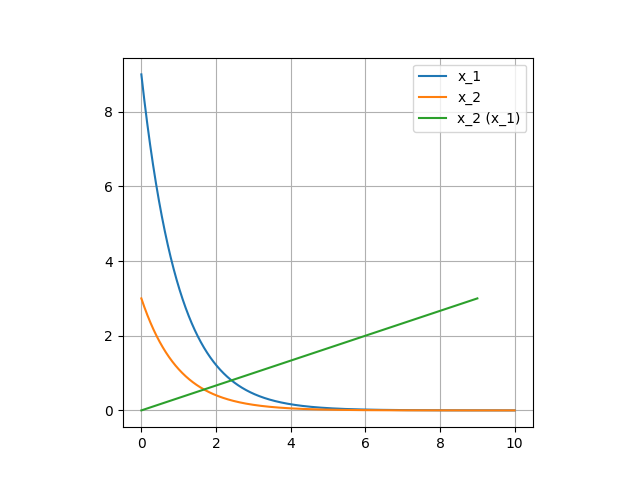
\includegraphics[width=0.75\linewidth]{pic/1_x0_3.png}}
\caption{Моделирование при $x_0 = \begin{pmatrix} 9 \\ 3 \end{pmatrix}$.}
\end{figure}
\begin{figure}[h!]
\center{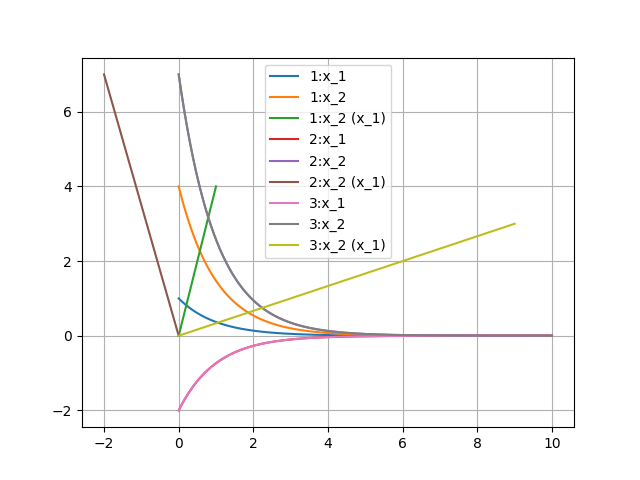
\includegraphics[width=1\linewidth]{pic/1_all.png}}
\caption{Моделирование 1 при $1: \, x_0 = \begin{pmatrix} 1 \\ 4 \end{pmatrix}$, $2: \, x_0 = \begin{pmatrix} -2 \\ 7 \end{pmatrix}$, $3: \, x_0 = \begin{pmatrix} 9 \\ 3 \end{pmatrix}$.}
\end{figure}
\newpage
На приведенных выше графиках проиллюстрирована асимптотически устойчивая система, ведь $\lim \limits_{t \to \infty} x_1 (t) = 0$ и $\lim \limits_{t \to \infty} x_2 (t) = 0$.

% part 2

\newpage
\subsection{}
\textit{Система неустойчива, при этом у матрицы $A$ не существует двух неколлинеарных собственных векторов.}
\begin{equation}
A=
\begin{pmatrix}
4 & 1\\
0 & 4
\end{pmatrix}
\end{equation}
\begin{figure}[h!]
\center{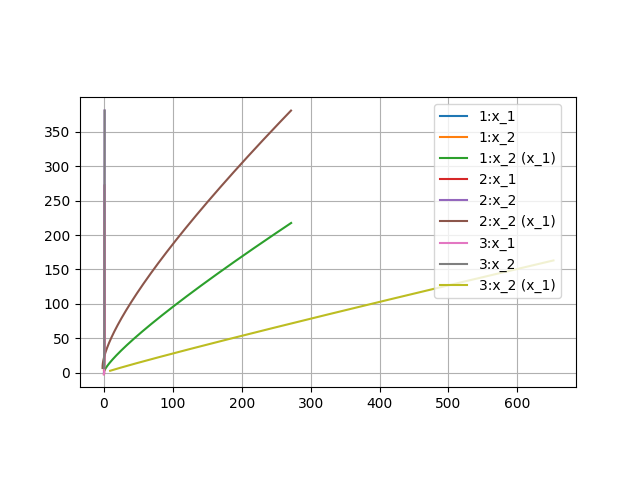
\includegraphics[width=1\linewidth]{pic/2_all.png}}
\caption{Моделирование 2 при  $1: \, x_0 = \begin{pmatrix} 1 \\ 4 \end{pmatrix}$, $2: \, x_0 = \begin{pmatrix} -2 \\ 7 \end{pmatrix}$, $3: \, x_0 = \begin{pmatrix} 9 \\ 3 \end{pmatrix}$.}
\end{figure}

Заметим, что система является неустойчивой, так как существуют такие начальные условия, что $\lim \limits_{t \to \infty} x_1 (t) = \infty$ и $\lim \limits_{t \to \infty} x_2 (t) = \infty$.

% part 3
\subsection{}
\textit{Система неустойчива, при этом если $x(0) = v_1$, то $\lim\limits_{t \to \infty} x(t) = 0$.}
\begin{equation}
A=
\begin{pmatrix}
0 & -1\\
-16 & 0
\end{pmatrix}
\end{equation}
\begin{figure}[h!]
\center{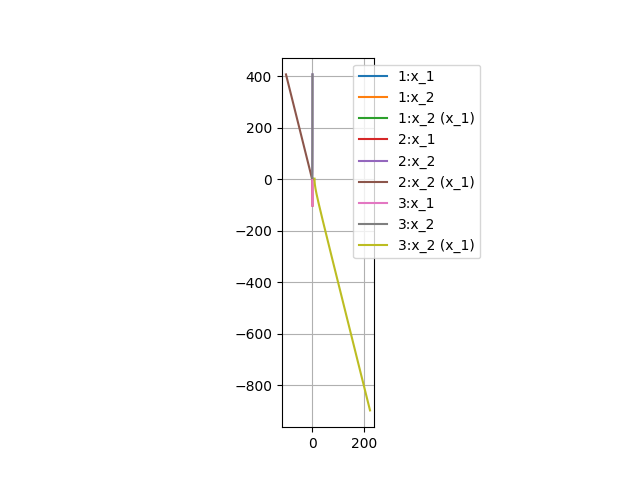
\includegraphics[width=1\linewidth]{pic/3_all.png}}
\caption{Моделирование 3 при  $1: \, x_0 = \begin{pmatrix} 1 \\ 4 \end{pmatrix}$, $2: \, x_0 = \begin{pmatrix} -2 \\ 7 \end{pmatrix}$, $3: \, x_0 = \begin{pmatrix} 9 \\ 3 \end{pmatrix}$.}
\end{figure}
\begin{figure}[h!]
\center{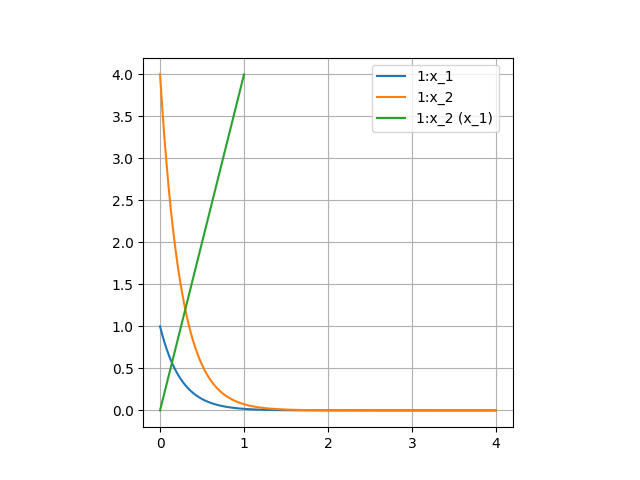
\includegraphics[width=1\linewidth]{pic/3_1.png}}
\caption{Моделирование 3 при  $ x_0 = \begin{pmatrix} 1 \\ 4 \end{pmatrix}$.}
\end{figure}
\newpage
Система неустойчива в общем случае, но при $x(0) = \begin{pmatrix} 1 \\ 4 \end{pmatrix}$,  $\lim\limits_{t \to \infty} x(t) = 0$


% part 4
\newpage
\subsection{}
\textit{Система асимптотически устойчива, при этом матрица $A \in \mathbb{R}^2$ имеет комплексные собственные вектора вида $v_1 \pm v_2 i \in \mathbb{C}^2$.}
\begin{equation}
A =
\begin{pmatrix}
1 & -1  \\
5 & -3
\end{pmatrix}
\end{equation}
\begin{figure}[h!]
\center{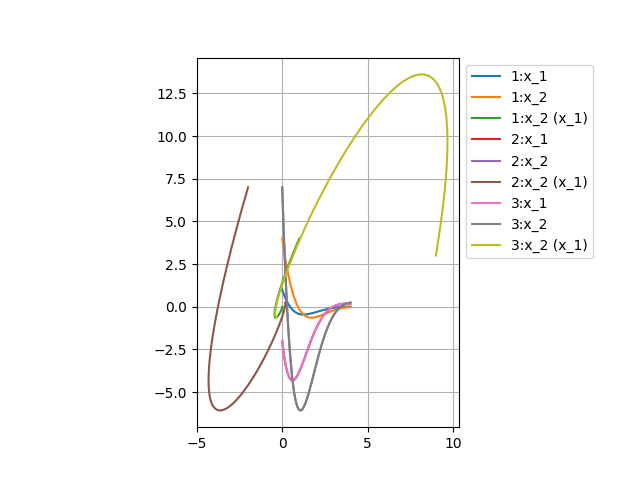
\includegraphics[width=1\linewidth]{pic/4_all.png}}
\caption{Моделирование 4 при  $1: \, x_0 = \begin{pmatrix} 1 \\ 4 \end{pmatrix}$, $2: \, x_0 = \begin{pmatrix} -2 \\ 7 \end{pmatrix}$, $3: \, x_0 = \begin{pmatrix} 9 \\ 3 \end{pmatrix}$.}
\end{figure}
\begin{figure}[h!]
\center{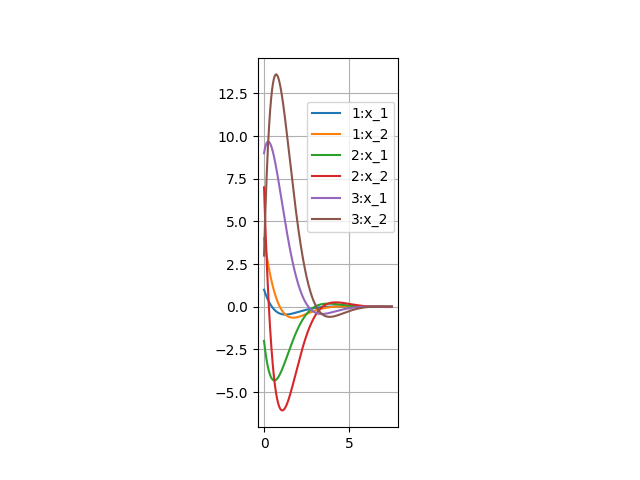
\includegraphics[width=1\linewidth]{pic/4_x_1.png}}
\caption{Моделирование 4, только зависимости $x(t)$,\\ при  $1: \, x_0 = \begin{pmatrix} 1 \\ 4 \end{pmatrix}$, $2: \, x_0 = \begin{pmatrix} -2 \\ 7 \end{pmatrix}$, $3: \, x_0 = \begin{pmatrix} 9 \\ 3 \end{pmatrix}$.}
\end{figure}
\newpage
Полученные графики подтверждают асимптотическую устойчивость системы, $\lim \limits_{t \to \infty} x_1 (t) = 0$ и $\lim \limits_{t \to \infty} x_2 (t) = 0$.


% part 5
\newpage
\subsection{}
\textit{Система неустойчива, при этом матрица $A$ имеет такие же собственные вектора, как в предыдущем пункте.}
\begin{equation}
A =
\begin{pmatrix}
3 & -1  \\
5 & -1
\end{pmatrix}
\end{equation}

\begin{figure}[h!]
\center{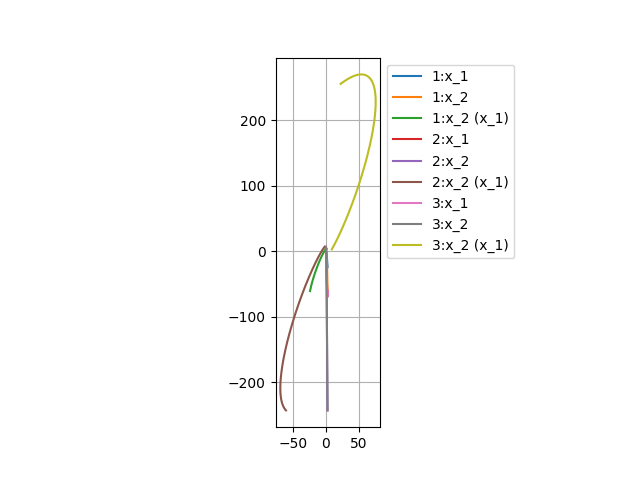
\includegraphics[width=1\linewidth]{pic/5_all.png}}
\caption{Моделирование 5 при  $1: \, x_0 = \begin{pmatrix} 1 \\ 4 \end{pmatrix}$, $2: \, x_0 = \begin{pmatrix} -2 \\ 7 \end{pmatrix}$, $3: \, x_0 = \begin{pmatrix} 9 \\ 3 \end{pmatrix}$.}
\end{figure}
\begin{figure}[h!]
\center{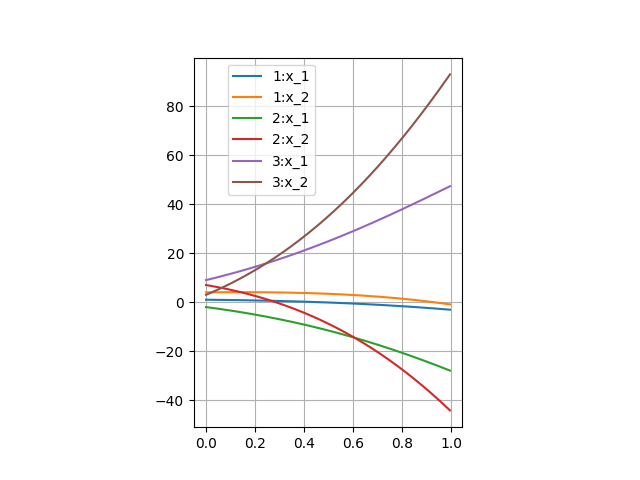
\includegraphics[width=1\linewidth]{pic/5_x.png}}
\caption{Моделирование 5, только зависимости $x(t)$, \\при  $1: \, x_0 = \begin{pmatrix} 1 \\ 4 \end{pmatrix}$, $2: \, x_0 = \begin{pmatrix} -2 \\ 7 \end{pmatrix}$, $3: \, x_0 = \begin{pmatrix} 9 \\ 3 \end{pmatrix}$.}
\end{figure}

\newpage
Заметим, что система действительно является неустойчивой, так как кривые $x_1(t), \, x_2(t)$ стремятся к $-\infty$ для заданных начальных условий.

% part 6
\newpage
\subsection{}
\textit{Система не является асимптотически устойчивой, но не является и неустойчивой, при этом матрица $A$ имеет собственные векторы такие же, как в пункте 4.}
\begin{equation}
A =
\begin{pmatrix}
2 & -1  \\
5 & -2
\end{pmatrix}
\end{equation}

\begin{figure}[h!]
\center{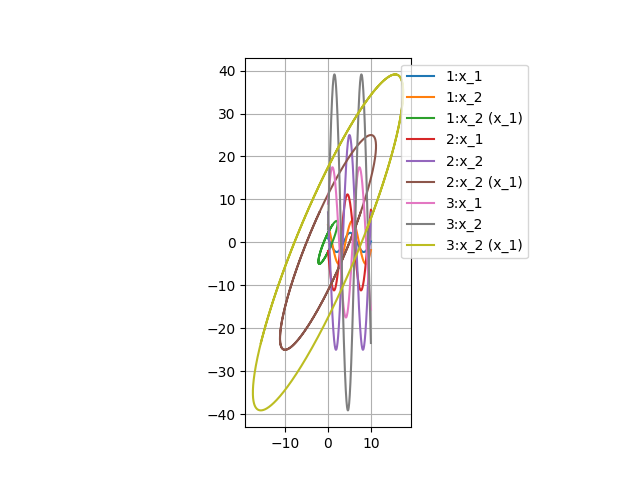
\includegraphics[width=1\linewidth]{pic/6_all_1.png}}
\caption{Моделирование 6 при  $1: \, x_0 = \begin{pmatrix} 1 \\ 4 \end{pmatrix}$, $2: \, x_0 = \begin{pmatrix} -2 \\ 7 \end{pmatrix}$, $3: \, x_0 = \begin{pmatrix} 9 \\ 3 \end{pmatrix}$.}
\end{figure}

\begin{figure}[h!]
\center{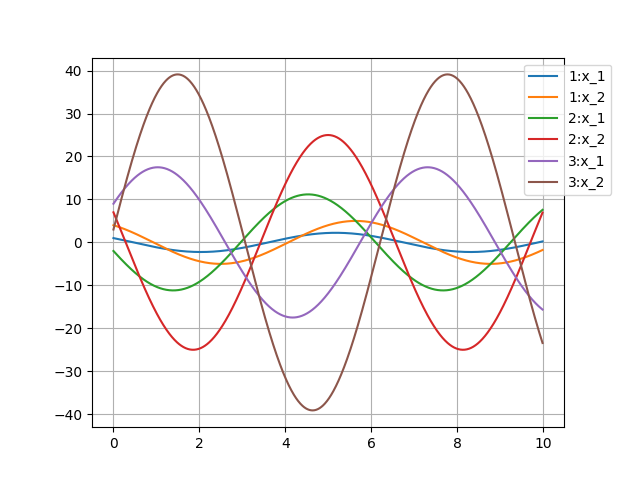
\includegraphics[width=1\linewidth]{pic/6_x.png}}
\caption{Моделирование 6, только зависимости $x(t)$, \\при  $1: \, x_0 = \begin{pmatrix} 1 \\ 4 \end{pmatrix}$, $2: \, x_0 = \begin{pmatrix} -2 \\ 7 \end{pmatrix}$, $3: \, x_0 = \begin{pmatrix} 9 \\ 3 \end{pmatrix}$.}
\end{figure}

\begin{figure}[h!]
\center{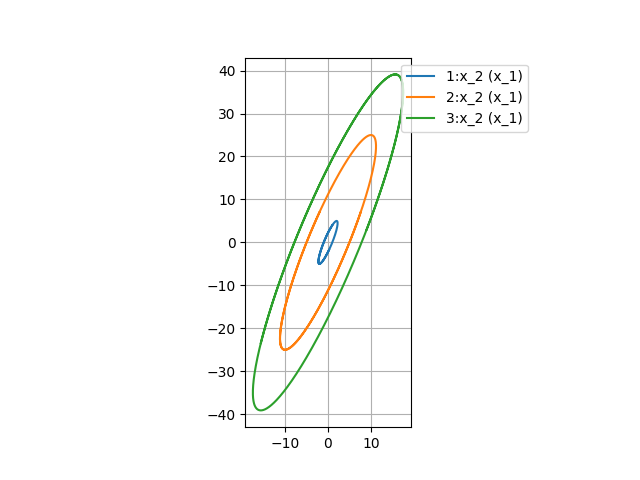
\includegraphics[width=1\linewidth]{pic/6_t.png}}
\caption{Моделирование 6, только зависимости $x_2(x_1)$, \\при  $1: \, x_0 = \begin{pmatrix} 1 \\ 4 \end{pmatrix}$, $2: \, x_0 = \begin{pmatrix} -2 \\ 7 \end{pmatrix}$, $3: \, x_0 = \begin{pmatrix} 9 \\ 3 \end{pmatrix}$.}
\end{figure}

\newpage
\,
\newpage
Система является не является ни асимптотически устойчивой, ни неустойчивой. Во-первых, функции $x_1(t)$, $x_2(t)$ не стремятся ни к нулю, ни к бесконечности при $t \to \infty$, а траектории $x_2(x_1)$ замкнуты, значит система обладает просто устойчивостью.



%task 3
\newpage
\section{задание. Придумать дискретное.}
\textit{Придумать дискретные динамические системы, обладающие следующими собственными числами (при этом ни одна из придуманных матриц $A$ не должна быть диагональной}:

%part 1
\subsection{$\lambda_{1, 2} = -1$}

\begin{equation}
A =
\begin{pmatrix}
-1&1 \\
0& -1
\end{pmatrix}
\end{equation}


%part 2
\subsection{$\lambda_{1, 2} = -\frac{1}{\sqrt{2}} \pm \frac{1}{\sqrt{2}} i$}

\begin{equation}
\left( \lambda + \frac{1}{\sqrt{2}} - \frac{1}{\sqrt{2}} i \right)\left( \lambda + \frac{1}{\sqrt{2}} + \frac{1}{\sqrt{2}} i \right)=0
\end{equation}
\begin{equation}
\lambda \left( \lambda + \frac{1}{\sqrt{2}} + \frac{1}{\sqrt{2}} i \right) + \frac{1}{\sqrt{2}} \left( \lambda + \frac{1}{\sqrt{2}} + \frac{1}{\sqrt{2}} i \right) - \frac{1}{\sqrt{2}} i \left( \lambda + \frac{1}{\sqrt{2}} + \frac{1}{\sqrt{2}} i \right) =0
\end{equation}
\begin{equation}
  \lambda^2 + \frac{1}{\sqrt{2}}\lambda + \frac{1}{\sqrt{2}} i\lambda + \lambda\frac{1}{\sqrt{2}} + \frac{1}{\sqrt{2}}  \frac{1}{\sqrt{2}} + \frac{1}{\sqrt{2}} \frac{1}{\sqrt{2}} i  - \frac{1}{\sqrt{2}} i\lambda - \frac{1}{\sqrt{2}} i \frac{1}{\sqrt{2}} - \frac{1}{\sqrt{2}} i \frac{1}{\sqrt{2}} i  =0
\end{equation}

\begin{equation}
  \lambda^2 + \frac{2\lambda}{\sqrt{2}} + 1  =0
\end{equation}
\begin{equation}
 \left( \lambda^2 + \frac{2\lambda}{\sqrt{2}} + \frac{1}{2} \right) + \frac{1}{2}  =0
\end{equation}
\begin{equation}
 \left( \lambda + \frac{1}{\sqrt{2}} \right)^2 + \frac{1}{2}  =0
\end{equation}
Искомая матрица:
\begin{equation}
A =
\begin{pmatrix}
-\frac{1}{\sqrt{2}} & -\frac{1}{2} \\
\\
1 & -\frac{1}{\sqrt{2}}
\end{pmatrix}
\end{equation}


%part 3
\subsection{$\lambda_{1, 2} = \pm i$}

\begin{equation}
\left( \lambda +  i \right)\left( \lambda - i \right)=0
\end{equation}

\begin{equation}
\lambda^2 +  1 =0
\end{equation}
Пусть искомая матрица имеет вид:
\begin{equation}
A =
\begin{pmatrix}
a & c \\
1 & b
\end{pmatrix}
\end{equation}
Тогда характеристический полином:
\begin{equation}
\left( a - \lambda \right) \left( b - \lambda \right) - c = 0
\end{equation}
\begin{equation}
\lambda^ 2 - \lambda (a + b ) + ab - c = \lambda^2 +  1 =0
\end{equation}

\begin{equation}
\begin{cases}
a = -b\\
ab - c = 1
\end{cases}
\to
\begin{cases}
a = -b\\
-a^2 - c = 1
\end{cases}
\end{equation}
Пусть $ a = 1$, тогда $b = -1$, $c = -2$.\\
Искомая матрица:
\begin{equation}
A =
\begin{pmatrix}
1 & -2 \\
1 & -1
\end{pmatrix}
\end{equation}

%part 4
\subsection{$\lambda_{1, 2} = \frac{1}{\sqrt{2}} \pm \frac{1}{\sqrt{2}} i$}

\begin{equation}
\left( \lambda -  \frac{1}{\sqrt{2}} - \frac{1}{\sqrt{2}} i \right) \left( \lambda -  \frac{1}{\sqrt{2}} + \frac{1}{\sqrt{2}} i  \right) = 0
\end{equation}
\begin{equation}
 \lambda\left( \lambda -  \frac{1}{\sqrt{2}} + \frac{1}{\sqrt{2}} i  \right) -  \frac{1}{\sqrt{2}}\left( \lambda -  \frac{1}{\sqrt{2}} + \frac{1}{\sqrt{2}} i  \right) - \frac{1}{\sqrt{2}} i \left( \lambda -  \frac{1}{\sqrt{2}} + \frac{1}{\sqrt{2}} i  \right) = 0
\end{equation}
\begin{equation}
\lambda^2 -  \frac{ \lambda}{\sqrt{2}} + \frac{ \lambda}{\sqrt{2}} i  -  \frac{\lambda}{\sqrt{2}} +  \frac{1}{2} - \frac{1}{2} i  - \frac{ \lambda}{\sqrt{2}} i  +  \frac{1}{2}i + \frac{1}{2}= 0
\end{equation}
\begin{equation}
\lambda^2 -  \frac{ 2 \lambda}{\sqrt{2}} + 1= 0
\end{equation}
\begin{equation}
\left( \lambda^2 -  \frac{ 2 \lambda}{\sqrt{2}} + \frac{1}{2} \right) + \frac{1}{2}= 0
\end{equation}
\begin{equation}
\left( \lambda -  \frac{ 1}{\sqrt{2}} \right)^2  + \frac{1}{2}= 0
\end{equation}
Искомая матрица:
\begin{equation}
A =
\begin{pmatrix}
 \frac{ 1}{\sqrt{2}} &  \frac{1}{2} \\
\\
-1 &  \frac{ 1}{\sqrt{2}}
\end{pmatrix}
\end{equation}



%part 5
\subsection{$\lambda_{1, 2} = 1$}

\begin{equation}
\left( \lambda - 1  \right)^2 = \lambda^2 - 2\lambda + 1 = 0
\end{equation}
Пусть искомая матрица имеет вид:
\begin{equation}
A =
\begin{pmatrix}
a & c \\
1 & b
\end{pmatrix}
\end{equation}

Тогда характеристический полином:
\begin{equation}
\left( a - \lambda \right) \left( b - \lambda \right) - c = 0
\end{equation}
\begin{equation}
\lambda^ 2 - \lambda (a + b ) + ab - c = \lambda^2 - 2\lambda + 1 = 0
\end{equation}
\begin{equation}
\begin{cases}
a + b = 2\\
ab - c = 1
\end{cases}
\end{equation}
Пусть $a = \frac{1}{2}$, $b = \frac{3}{2}$, тогда $c = -\frac{1}{4}$. \\
\\
Искомая матрица:
\begin{equation}
A =
\begin{pmatrix}
 \frac{1}{2} &   -\frac{1}{4}\\
\\
1 & \frac{3}{2}
\end{pmatrix}
\end{equation}

\newpage
\textbf{Для следующих пунктов выберем константы: $c = \frac{1}{2}$, $d = 2$.}
\\

%part 6
\subsection{$\lambda_{1, 2} = -\frac{1}{2}$}

\begin{equation}
A =
\begin{pmatrix}
 -\frac{1}{2} &  1\\
\\
0 &  -\frac{1}{2}
\end{pmatrix}
\end{equation}

%part 7
\subsection{$\lambda_{1, 2} = \pm \frac{i}{2}$}

\begin{equation}
\left( \lambda +  \frac{i}{2} \right)\left( \lambda - \frac{i}{2} \right)=0
\end{equation}

\begin{equation}
\lambda^2 +  \frac{1}{4} =0
\end{equation}
Пусть искомая матрица имеет вид:
\begin{equation}
A =
\begin{pmatrix}
a & c \\
1 & b
\end{pmatrix}
\end{equation}
Тогда характеристический полином:
\begin{equation}
\left( a - \lambda \right) \left( b - \lambda \right) - c = 0
\end{equation}
\begin{equation}
\lambda^ 2 - \lambda (a + b ) + ab - c = \lambda^2 +  \frac{1}{4} =0
\end{equation}

\begin{equation}
\begin{cases}
a = -b\\
ab - c = \frac{1}{4} 
\end{cases}
\to
\begin{cases}
a = -b\\
-a^2 - c = \frac{1}{4} 
\end{cases}
\end{equation}
Пусть $ a = 1$, тогда $b = -1$, $c = -\frac{5}{4} $.\\
Искомая матрица:
\begin{equation}
A =
\begin{pmatrix}
1 &  -\frac{5}{4}  \\
\\
1 & -1
\end{pmatrix}
\end{equation}



%part 8
\subsection{$\lambda_{1, 2} = \frac{1}{2}$}

\begin{equation}
\left( \lambda - \frac{1}{2}  \right)^2 = \lambda^2 - \lambda + \frac{1}{4} = 0
\end{equation}
Пусть искомая матрица имеет вид:
\begin{equation}
A =
\begin{pmatrix}
a & c \\
1 & b
\end{pmatrix}
\end{equation}

Тогда характеристический полином:
\begin{equation}
\left( a - \lambda \right) \left( b - \lambda \right) - c = 0
\end{equation}
\begin{equation}
\lambda^ 2 - \lambda (a + b ) + ab - c = \lambda^2 - \lambda + \frac{1}{4} = 0
\end{equation}
\begin{equation}
\begin{cases}
a + b = 1\\
ab - c =  \frac{1}{4}
\end{cases}
\end{equation}
Пусть $a = \frac{1}{4}$, $b = \frac{3}{4}$, тогда $c = -\frac{1}{16}$. \\
\\
Искомая матрица:
\begin{equation}
A =
\begin{pmatrix}
  \frac{1}{4} &  -\frac{1}{16}\\
\\
1 & \frac{3}{4}
\end{pmatrix}
\end{equation}





%part 9
\subsection{$\lambda_{1, 2} = -2$}

\begin{equation}
A =
\begin{pmatrix}
 -2 &  1\\
\\
0 &  -2
\end{pmatrix}
\end{equation}


%part 10
\subsection{$\lambda_{1, 2} = \pm 2i$}

\begin{equation}
\left( \lambda +  2i \right)\left( \lambda - 2i \right)=0
\end{equation}

\begin{equation}
\lambda^2 +  4 =0
\end{equation}
Пусть искомая матрица имеет вид:
\begin{equation}
A =
\begin{pmatrix}
a & c \\
1 & b
\end{pmatrix}
\end{equation}
Тогда характеристический полином:
\begin{equation}
\left( a - \lambda \right) \left( b - \lambda \right) - c = 0
\end{equation}
\begin{equation}
\lambda^ 2 - \lambda (a + b ) + ab - c =\lambda^2 +  4 =0
\end{equation}

\begin{equation}
\begin{cases}
a = -b\\
ab - c = 4
\end{cases}
\to
\begin{cases}
a = -b\\
-a^2 - c = 4
\end{cases}
\end{equation}
Пусть $ a = 1$, тогда $b = -1$, $c = -5 $.\\
Искомая матрица:
\begin{equation}
A =
\begin{pmatrix}
1 &  -5  \\
1 & -1
\end{pmatrix}
\end{equation}


%part 11
\subsection{$\lambda_{1, 2} = 2$}
\begin{equation}
A =
\begin{pmatrix}
 2 &  1\\
0 &  2
\end{pmatrix}
\end{equation}


%part 12
\subsection{$\lambda_{1, 2} = 0$}
\begin{equation}
A =
\begin{pmatrix}
 0 &  1  \\
0 & 0
\end{pmatrix}
\end{equation}


%task 4
\newpage
\section{задание. Замоделировать дискретное.}


\end{document}













